\chapter{Les sons - Modèle de perception}
\section{Introduction}
\subsection{Définitions}
\begin{itemize}
    \item \textbf{Psychophysique} : relation entre le \textit{stimulus}\footnote{Phénomène physique} et la \textit{sensation} ressentie du stimulus. \newline
    \item \textbf{Psychoacoustique} \footnote{Remarque : on peut tromper l'ouie comme la vue, avec des sons appelés \textbf{sons de Risset}} : étude de la relation entre les vibrations des ondes sonores et sa perception.\newline
    \item \textbf{Les modèles de production} permettent de caractériser les osurces dans la nature.
\end{itemize}
\subsection{Histoire des sens} \footnote{D'après Ch. Sherrington (1857-1952)}
\begin{itemize}
    \item Les sens \textit{introseptifs} : sensations qui vienne des entrailles du corps (estomac, coeur, malaise, aise...)
    \item Les sens \textit{Proprioceptifs} : 
        \begin{itemize}
            \item Sens \textit{statique} ou \textit{labyrinthique}\footnote{Provient du "capteur" situé dans l'oreille interne} : mouvements de rotation et de translation
            \item Sens \textit{kinésique} ou \textit{kinestésique} : permet la perception des objets dans l'espace, par exemple le toucher
        \end{itemize}
    \item Les sens \textit{extéroceptifs}
        \begin{itemize}
            \item Sens par contact direct
                \begin{itemize}
                    \item Le \textit{toucher}
                    \item Les sens \textit{chimique} : goût, odorat
                \end{itemize}
            \item Sens par contact indirect
                \begin{itemize}
                    \item \textit{Vue}
                    \item \textit{Ouie}
                \end{itemize}
        \end{itemize}
\end{itemize}
\newpage
\subsection{Lois des sens (18ème - 19ème)}
\begin{itemize}
    \item \textbf{Loi du sens} : il existe pour chaque sens une intensité minima du stimulus, appelée intensité liminaire, au-dessous de laquelle il n'y a pas de sensation
    \item \textbf{Loi du seuil différentiel} : 
        \begin{itemize}
            \item Forme a. \newline
            Il existe un rapport constant entre l'intensité du stimulus initial et la variation minima qu'il faut lui faire subir pour que la différence soit sentie
            \item Forme b. \newline
            Pour que la sensation subisse des accroissements en progression arithmétique (0, 1, 2...), il faut faire varier le stimulus en progression géométrique (a, a2, a3...) ; le rapport constant est le seuil liminaire. C'est encore la loi logarithmique, ou loi de Fechner
        \end{itemize}
\end{itemize}
\newpage
\section{Stimulus auditif : le son}
\subsection{Qu'est-ce que le son ?}
C'est la sensation perçue par l'oreille. Variation périodique de la pression d'un milieu.
\subsection{Hypothèses du cours}
\begin{itemize}
    \item Millieux de propagation \footnote{(gazs, liquides, solides)} supposés parfaits, sans viscosité et au repos \footnote{En réalite, pour les fluides visqueux, on doit résoudre l'équation de Navier-Stokes par la méthode des éléments finis}
    \item Vibrations de faible amplitude
    \item Transformations des fluides supposés adiabatiques réversibles
\end{itemize}
\section{Equation d'ondes}
\subsection{Unidimensionnel}
Equation de propagation des ondes électro-magnétiques :
\begin{equation}
    \large
    \tcbhighmath[fuzzy halo=0.5mm with electricultramarine!35!electricultramarine,arc=2pt,
    boxrule=0pt,frame hidden]{ 
        \frac{\partial^{2} \psi}{\partial t^{2}} = c_{s}^{2}\frac{\partial^{2} \psi}{\partial x^{2}}
    } \label{eq propagation}
    \normalsize
\end{equation}
et : 
\begin{equation}
    \label{eq 1}
    \rho_{e} = -\rho_{0}\frac{\partial \psi }{\partial x}  
\end{equation}
\begin{equation}
    \label{eq 2}
    P_{e} = c_{s}^{2}\rho_{e}
\end{equation}
\begin{equation}
    \label{eq 3}
    \rho_{0} \frac{\partial^{2} \psi}{\partial t^{2}} = -\frac{\partial P_{e}}{\partial x}
\end{equation}
Ce qui devient pour l'équation d'ondes sonores :
\begin{equation}
    \Large
    \tcbhighmath[fuzzy halo=0.5mm with electricultramarine!35!electricultramarine,arc=2pt,
    boxrule=0pt,frame hidden]{ 
        \frac{\partial^{2} P_{e}}{\partial t^{2}} = \frac{1}{c_{s}^{2}}\frac{\partial^{2} P_{e}}{\partial x^{2}}
     } \nonumber
    \normalsize
\end{equation}
\vfil
\begin{equation}
    \small
    \tcbhighmath[fuzzy halo=0.5mm with electricultramarine!35!electricultramarine,arc=2pt,
    boxrule=0pt,frame hidden]{ 
        c_{s} = 331,4\sqrt{1+\frac{T}{T_{0}}} = \sqrt{\frac{dP(\rho_{0})}{d\rho}}
     } \nonumber
    \normalsize
\end{equation}
\vfill
\begin{center}
    \small{Pour démonstration voir annexe \ref{Annexe 1}}
\end{center}
\newpage
\subsection{Tridimensionnel}
L'équation d'ondes s'écrit à l'aide du d'Alembertien : 
\begin{definition}{D'Alembertien}{d'Alembertien}
    \[ \Xi = \nabla^{2} - \frac{1}{c_{2}^{2}}\frac{\partial^{2}}{\partial t^{2}} \]
\end{definition}
Comme on a $\Xi P_{e} = 0$, on peut écrire l'équation d'onde suivante :
\begin{equation}
    \large
    \tcbhighmath[fuzzy halo=0.5mm with electricultramarine!35!electricultramarine,arc=2pt,
    boxrule=0pt,frame hidden]{ 
        \nabla^{2}P_{e} - \frac{1}{c_{2}^{2}}\frac{\partial^{2} P_{e}}{\partial t^{2}} = 0 \nonumber
     } \nonumber
    \normalsize
\end{equation}
Avec : \newline
\large
\begin{itemize}
    \item $\nabla^{2}\psi = \Delta \psi = \frac{\partial^{2} \psi}{\partial x^{2}} + \frac{\partial^{2} \psi}{\partial y^{2}} + \frac{\partial^{2} \psi}{\partial z^{2}} + \frac{\partial^{2} \psi}{\partial t^{2}}$ \newline
    \item $\psi$ : fonction d'onde (électromagnétique) \newline
    \item $c_{s}$ : célérité du son dans l'air en $m.s^{-1}$ ($c_{s} \approx 340 m.s^{-1}$) \newline
    \item $c$ : célérité de la lumière, $c\approx 3.10^{8}m.s^{-1}$ \newline
    \item $P_{e}$ : pression acoustique en $Pa$ \newline
    \item $T$ : température en $C$ \newline
    \item $T_{0} = 273 C$ \newline
    \item $k = ||\vec{k}||$ : norme du vecteur d'ondes \newline
    \item $\omega = 2\pi f = \frac{2\pi}{T}$ : pulsation d'onde en $rad.s^{-1}$ \newline
    \item $f$ : fréquence de l'onde en $Hz$ \newline
    \item $T$ : période de l'onde en $s$ \newline
    \item $\phi$ : déphasage en $rad$
\end{itemize}
\normalsize
\newpage
\section{Solutions de l'équation d'ondes}
\subsection{Solution pour une onde plane progressive monochromatique (OPPM)}
En considérant l'onde comme une OPPM dans un milieu homogène et isotrope, constitué d'air assimilé à un gaz parfait, on a la relation suivante $k = \frac{\omega}{c}$ qui provient de l'équation \eqref{eq propagation}. On a alors :
\begin{align}
    \psi(x,t) &= Acos(\omega t - \vec{k}.\vec{x}) \\ \nonumber
        &= Acos(\omega(t - \frac{x}{c})) \nonumber
\end{align}
Ce qui donne pour les ondes sonores :
\begin{equation}
    \large
    \tcbhighmath[fuzzy halo=0.5mm with electricultramarine!35!electricultramarine,arc=2pt,
    boxrule=0pt,frame hidden]{ 
        P(x,t) = Acos(k(x - c_{s}t) + \phi)
     } \nonumber
    \normalsize
\end{equation}
Avec $k=\frac{\omega}{c_{s}}$
\subsection{Solution pour une onde stationnaire}
Les ondes stationnaires proviennent de la superposition d'une onde provenant d'une source et de cette même onde réfléchie sur un conducteur, que l'on considère parfait, c'est-à-dire de conductivité nulle. On considère aussi que le problème est suffisament bien posé pour que le théorème de superposition soit applicable. Il vient 
\begin{equation}
    \phi(x,t)=\phi(x)=\phi_{1}(x)+\phi_{2}(x)
\end{equation}
Soit :
\begin{equation}
    \large
    \tcbhighmath[fuzzy halo=0.5mm with electricultramarine!35!electricultramarine,arc=2pt,
    boxrule=0pt,frame hidden]{ 
        P(x,t) = Acos(kx + \phi)sin(\omega t + \phi')
     } \nonumber
    \normalsize
\end{equation}
\subsection{Ondes stationnaires pour deux parois rigides}
On considère un milieu homogène constitué de deux parois rigides séparés d'une distance $L$, rempli d'air entre les deux parois, toujours assimilé à un gaz parfait.
\begin{equation}
    \normalsize
    \tcbhighmath[fuzzy halo=0.5mm with electricultramarine!35!electricultramarine,arc=2pt,
    boxrule=0pt,frame hidden]{ 
        P(x,t) = \sum_{n=0}^{+\infty}{A_{n}cos(n\pi \frac{x}{L})cos(n\pi \frac{ct}{L} + \phi_{n}')}
     } \nonumber
    \normalsize
\end{equation}
\subsection{Ondes stationnaires pour deux parois molles}
On considère un milieu homogène constitué de deux parois molles séparés d'une distance $L$, rempli d'air entre les deux parois, toujours assimilé à un gaz parfait.
\begin{equation}
    \normalsize
    \tcbhighmath[fuzzy halo=0.5mm with electricultramarine!35!electricultramarine,arc=2pt,
    boxrule=0pt,frame hidden]{ 
        P(x,t) = \sum_{n=0}^{+\infty}{A_{n}cos(n\pi \frac{x}{L} + \frac{\pi}{2})cos(n\pi \frac{ct}{L} + \phi_{n}')}
     } \nonumber
    \normalsize
\end{equation}
\vfill
\begin{center}
    \small
    Pour plus de précisions, voir annexe \Ref{annexe2}
    \normalsize
\end{center}
\newpage
\subsection{Ondes stationnaires pour une paroi molle et une paroi rigide}
Les deux parois sont toujours espacées d'une distance $L$
\begin{equation}
    \normalsize
    \tcbhighmath[fuzzy halo=0.5mm with electricultramarine!35!electricultramarine,arc=2pt,
    boxrule=0pt,frame hidden]{ 
        P(x,t) = \sum_{n=0}^{+\infty}{A_{n}cos((2n+1)\pi\frac{x}{2L} )cos((2n + 1)\pi \frac{ct}{2L} + \phi_{n}')}
     } \nonumber
    \normalsize
\end{equation}
\section{Un peu d'anatomie}
\subsection{Représentation des "capteurs" de l'Homme}
\begin{figure}[hbt!]
    \begin{subfigure}{.47\textwidth}
      \centering
      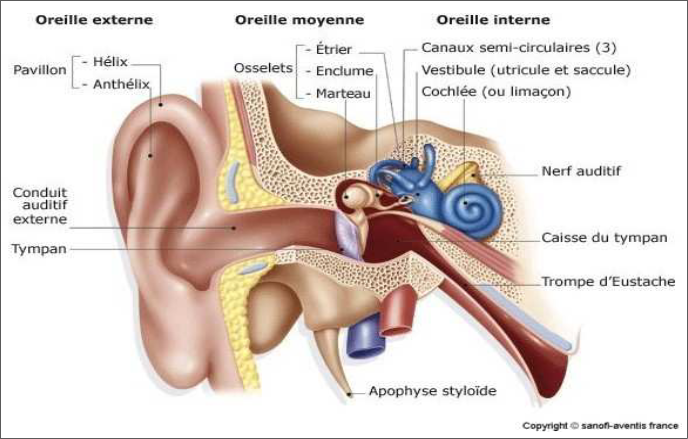
\includegraphics[width=.7\linewidth]{Pics/Oreille.png}
      \caption{Schéma d'une oreille}
      \label{fig:sfig1}
    \end{subfigure}%
    \begin{subfigure}{.55\textwidth}
      \centering
      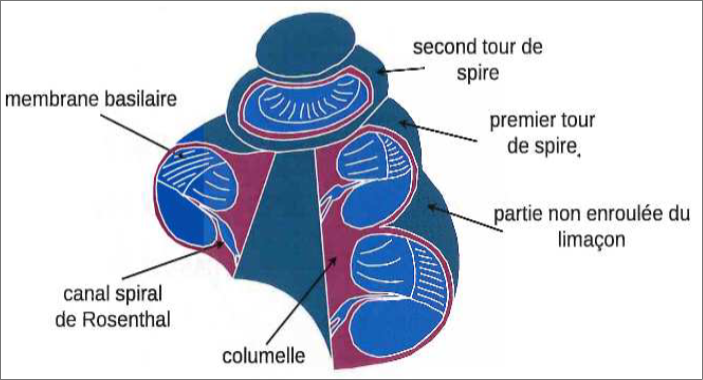
\includegraphics[width=.7\linewidth]{Pics/Cochlee.png}
      \caption{Schéma d'une cochlée}
      \label{fig:sfig2}
    \end{subfigure}
    \caption{Schéma des "capteurs" de l'Homme pour le son}
    \label{fig:fig}
\end{figure}
\begin{figure}[hbt!]
    \begin{subfigure}{.5\textwidth}
      \centering
      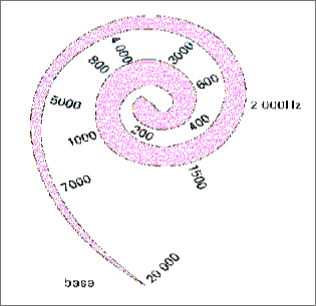
\includegraphics[width=.45\linewidth]{Pics/conv_position_freq.png}
      \caption{Conversion position fréquence chez la cochlée}
      \label{fig:sfig1}
    \end{subfigure}%
    \begin{subfigure}{.5\textwidth}
      \centering
      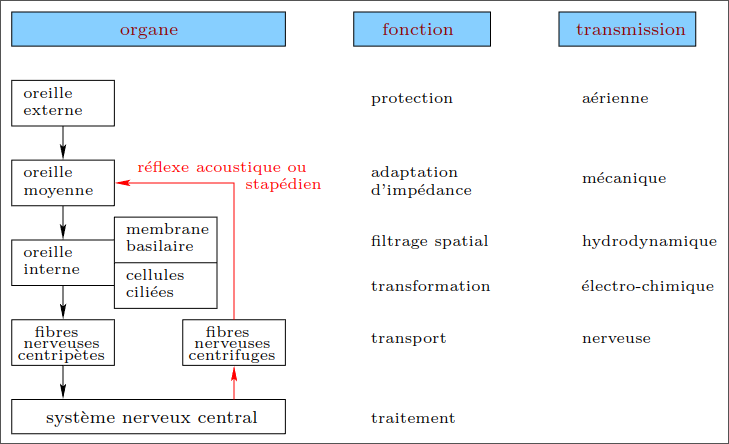
\includegraphics[width=.7\linewidth]{Pics/Transmission_Information_chez_lH.png}
      \caption{Transmission de l'information chez l'Homme}
      \label{fig:sfig2}
    \end{subfigure}
    \caption{Conversion de la grandeur physique à l'information}
    \label{fig:fig}
\end{figure}
\subsection{Influx nerveux}
L'influx nerveux est une variation de potentiel cellulaire pendant une durée d'environ $100ms$ qui ne varie pas en répétant l'expérience, quelque soit la sensation. Ces sensations sont localisées dans le cortex\footnote{zone du cerveau}, dans les zones de l'audition et de la vision
\newpage
\subsection{Phénomène acoustique des sensations}
\begin{itemize}
    \item \textbf{Perception de l'intensité} (énergie) du son \newline
        \begin{itemize}
            \item Le son sur un point fixe de coordonnées $(x,y)$ est décrit par la pression acoustique $p$ qui dépend du temps $t$, exprimée en $Pa$, $[Pa]=[\frac{N}{m^{2}}]$.
            \item Niveau de pression acoustique : 
            \begin{equation}
                \normalsize
                \tcbhighmath[fuzzy halo=0.5mm with electricultramarine!35!electricultramarine,arc=2pt,
                boxrule=0pt,frame hidden]{ 
                    L = 20log_{10}(\frac{p_{eff}}{p_{0}})
                } \nonumber
                \normalsize
            \end{equation}
            Avec : 
            \begin{itemize}
                \item $p_{eff}$ : pression acoustique efficace en $Pa$, $p_{eff_{max}} = 10^{2} Pa$
                \item $p_{0}$ : pression acoustique minimale audible, $p_{0} = 2.10^{-5} Pa$
            \end{itemize}
            \item Loi du seuil :
            \begin{figure}[hbt!]
                \centering
                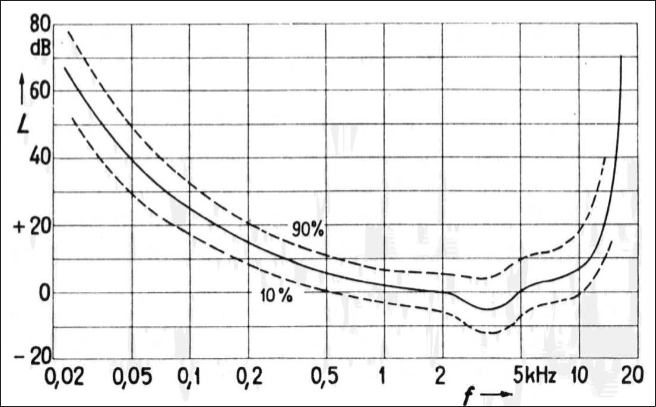
\includegraphics[scale=0.3]{Pics/Loi_du_Seuil.png}
                \caption{Loi du seuil : seuil de perception du son en fonction de l'intensité sonore et de la fréquence}
            \end{figure}
            \item COurbe d'isosonie :
            \begin{figure}[hbt!]
                \centering
                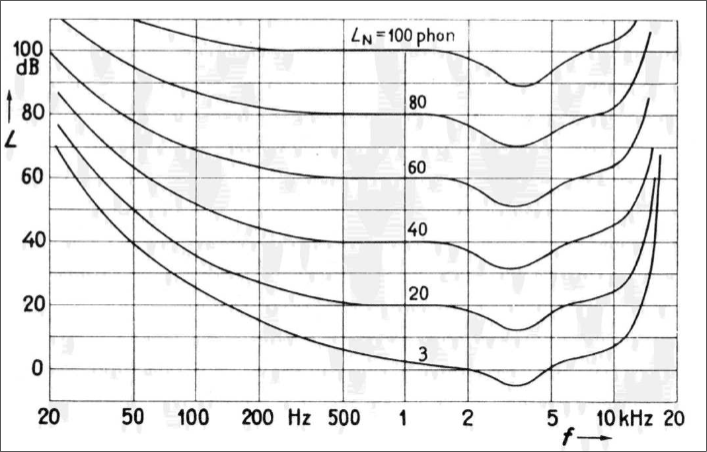
\includegraphics[scale=0.3]{Pics/Courbe_isosonie.png}
                \caption{Loi du seuil : seuil de perception du son en fonction de l'intensité sonore et de la fréquence}
            \end{figure}
        \end{itemize}
    \newpage
    \item \textbf{Perception de la hauteur} (fréquence des vibrations dans l'air) du son pur \newline
        \begin{itemize}
            \item \textbf{Bande critique}
            \item \textbf{Echelle des mels}
            
        \end{itemize}
    \item \textbf{Perception du timbre } : amplitude des sons accessoires et partiels \newline
    \item \textbf{Perception dans l'espace} : localisation de la source dans l'espace
\end{itemize}
\begin{figure}[hbt!]
    \centering
    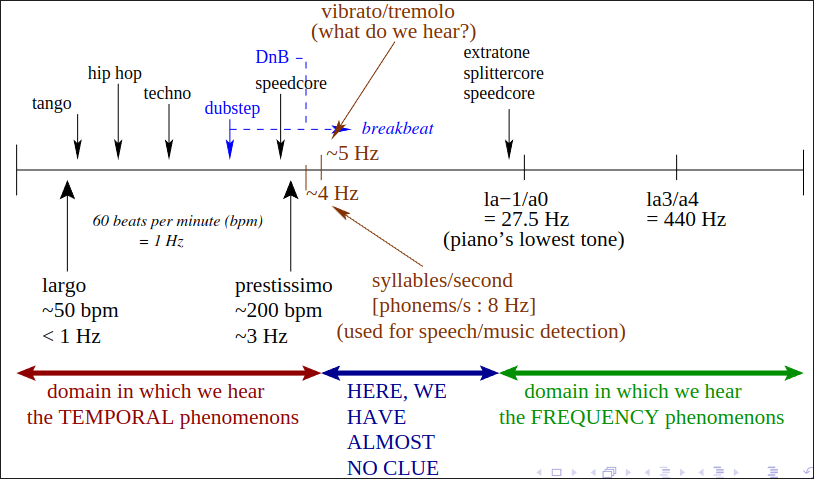
\includegraphics[scale=0.4]{Pics/Perception_bpm.png}
    \caption{Perception des sons chez l'Homme en fonction du bpm ($60 bmp$ correspond à $1 Hz$)}
\end{figure}